\chapter{Problem Analysis}
\label{problemanalysis}

In the scope of our project, all citations are classified into 2 types: \textbf{General} and \textbf{Specific}. We define citations as such to be inline with our goal. That is, to be able to tell if Specific, where the cited information is in the cited document. Otherwise, the citation would be deemed General. To rid of ambiguity in our definition of a General/Specific citation, we have the following guidelines: \\ \\
\textbf{General Citations}
\begin{enumerate}
\item Authors may refer to a paper as a whole. If the author cites for a key idea, e.g. Machine Learning, and Machine Learning makes up the entire or majority of the cited paper, it is a general citation.
\item Authors may refer to a paper as a form of mentioning. The authors merely mentions the cited paper out of acknowledgement of its contributions.
\end{enumerate}
\textbf{Specific Citations}
\begin{enumerate}
\item Authors may refer to a term definition in the cited paper.
\item Authors may refer to a key idea/implementation in the cited paper. This key idea/implementation does not make up the entire cited paper.
\item Authors may refer to an algorithm or a theorem in the cited paper. This algorithm/theorem does not make up the entire cited paper.
\item Authors may refer to digits or numerical figures in the cited paper. Usually for making reference to evaluation results in the cited paper. Authors may also complement the cited paper for its promising/excellent performance.
\item Authors may quote a line/segment in the cited paper.
\end{enumerate}

\begin{figure}[h]
\label{fig:terminology}
\framebox[\textwidth]{
	\begin{tabular}{ l p{11cm}}
		\textsc{Term} & \textsc{Description}\\
		\hline
		Citing Paper & The paper that makes the citation \\
		Cited Paper & The paper that is being cited by the citing paper \\
		Cite Link & E.g. \url{E06-1034==>J93-2004}. A citation relation between a citing paper (\url{E06-1034}) and a cited paper (\url{J93-2004}) \\
		Cite String & The citation mark. E.g. Nivre and Scholz (2004), [1], (23) \\
		Citing Sentence & A sentence in the citing paper that contains the in-line citation. E.g. \textit{That algorithm, in turn, is similar to the dependency parsing algorithm of \textbf{Nivre and Scholz (2004)}, but it builds a constituent tree and a dependency tree simultaneously.} \\
		Citing Context & The block of text surrounding the citing sentence, about 2 sentences before and after the citing sentence, for providing contextual information \\
		Cited Fragment & A fragment, from a few lines to paragraphs, in the cited paper
	\end{tabular}
}
\caption{Terminologies used in this paper}
\end{figure}

In general, for \textbf{Specific} citations, we would be able to specifically extract a fragment in the cited paper that represents the source of the information mentioned in the citation itself i.e. Citation Provenance.

\section{Scope Of The Problem}
I now reduce the problem to determining whether a citation is General or Specific. If a citation is General, the reader can be directed, for example, to the Abstract section of the cited paper. If a citation is Specific, the reader can be directed to that specific paragraph or lines respectively.
%Therefore during computation, the cited document can be broken down into fragments.
If given that a citation is Specific, then there must exists a region in the cited paper that the citation refers to. For this I need to implement some ranking system that determines the location of this region.

I abstract away the problem of locating the in-line citations in a paper, and reduce the problem to only determining the type of a citation and its location. To solve the problem of locating the in-line citations, I utilize the open-source ParsCit system developed by \cite{parscit}. Conveniently, ParsCit identifies the citing sentence, together with its citing context.

\section{Modelling The Problem As Search}
In web search engines, an user enters a search query, and a search engine would use this query to search within its search domain -- millions of web pages -- and then display the best matching web pages as compared to the search query. That would be equivalent to having a search query for an entire corpus of research papers. This problem can also be modelled as a searching problem, but a reduced version as compared to web search engines.

Consider reading a paper, \url{A}. We know the citations made by \url{A}, and these cited papers are listed in its References section. From this our search domain for any query from \url{A} would be the contents of the list of cited papers. We reduce this search domain further when we are investigating a particular citation in \url{A}, say now paper \url{A} cites the paper \url{B}. Now, for this citation, the scope of search would be the sub-domain -- contents of paper \url{B}. So instead of searching for the best matching document in the corpus, we are now searching within \url{B}. The search query is the citation from \url{A}, the {\it candidate documents} would be various regions (referred to as fragments) in \url{B} (Refer to Figure \ref{fig:model} for a simple illustration). With the help of ParsCit \cite{parscit}, the citing context can be extracted. The search query would be citing context which consists of the citing sentence.

\begin{figure}[h]
  \centering
  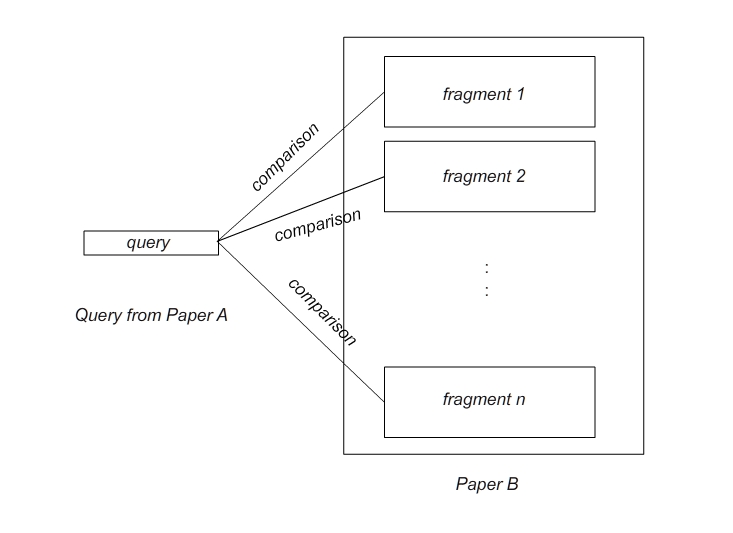
\includegraphics[scale=0.50]{./model}
  \caption{Modeling Our Problem}
  \label{fig:model}
\end{figure}

Our problem is now a \textit{binary classification problem}, where we attempt to determine whether a fragment is either General or Specific.

\section{Building Our Corpus}
\label{buildingcorpus}
At this initial stage, I picked the ACL Anthology Reference Corpus\footnote{http://acl-arc.comp.nus.edu.sg/} (ACL-ARC). The ACL-ARC consists of publications of the Computational Linguistics field. Note that in general, we wish to perform this citation provenance task on all publications from all fields of research. This corpus is chosen as a start, because it provides the \textit{interlink data} that conveniently informs us of the cite links between the papers in the corpus. For instance, in the interlink data, a link like \url{X98-103==>X96-1049} says that the paper \url{X98-103}\footnote{All ACL-ARC papers are assigned an unique paper ID} cites \url{X96-1049}.

Now that I have modelled our problem, I am able to specify the required data format for the task. For each cite link, there can be multiple in-line citations i.e. multiple citing contexts. Each citing context is compared with every fragment in the cited paper. In other words, if a cite link has $n$ citing contexts and the cited paper can be divided into $m$ fragments, immediately we have $(n \times m)$ data instances.

\subsection*{Collecting Annotations - First Attempt}
The first attempt at collecting annotations was to require an annotator to specify the line numbers of the cited information that the citing context was referring to. The annotator would be provided the citing and cited paper in plain text format, and he/she will need to annotate on a separate file, specifying the line number range, e.g. line range \url{L12-55} of the cited paper. For this annotation task, I designed an annotation framework\footnote{http://citprov.heroku.com} where an annotator is presented with an user-friendly interface to select the lines in the cited paper that he/she deem Specific. We posted this task onto the Amazon Mechanical Turk (MTurk\footnote{https://www.mturk.com}) as an attempt to collect annotations on a larger scale and I collected some annotations from a few MTurk workers. After a trial round of annotation, I reviewed this annotation scheme together with feedbacks from the small group of participants.

First, this annotation task is a non-trivial one. Participants must be able to understand the contents of the papers, thus, must be researchers or have some experience in reading scientific papers. While it is possible to target a selected category of MTurk workers for this task, the complexity of this task requires participants with research experiences, which could be limited in numbers. Furthermore, most of the annotations collected from MTurk do not agree among the annotators and ourselves. Thus I abandoned collecting annotations via MTurk, and performed annotations manually.

Second, this annotation scheme is too tricky, and would also cause us much problem when it comes to evaluation. Consider an implemented system that outputs a prediction for citation provenance in the form of a line number range. It is difficult to judge the correctness of this prediction, say \url{L50-78}, when compared against the annotated \url{L12-55}. The prediction \textit{overlaps} the annotation by 5 lines, but this variable amount of overlap is not definitive and difficult to decide at what extent of overlap only do we consider the prediction correct. Thus I switched to the alternative.

\subsection*{Collection Annotations - Second Attempt}
The second attempt is more straightforward. Recall that I use ParsCit for extracting the citing context. ParsCit also divides a paper into logically adequate fragments according to sections, sub-sections, figures and tables etc. So instead of annotating the papers in plain text format by line number ranges, I annotated the structured output from ParsCit, each of the fragments of the cited papers with 3 classes: General ($g$), Specific-Yes ($y$) and Specific-No ($n$). To be precise, I annotate $g$ (for all its fragments) if a cite link is deemed General, and $y$ \underline{only} for the fragment(s) that is deemed Specific. For the other fragments that are not Specific, I annotate $n$. Table \ref{tab:annotation} summarises the statistics for annotation. Note that only percentage values for Specific instances are displayed.

\begin{table}[h]
	\center
	\begin{tabular}{ l | l}
		\textsc{Item} & \textsc{Statistics}\\
		\hline
		No. of Cite Links & 275 (7.6\% Specific) \\
		No. of Fragments & 30943 (0.09\% Specific-Yes, 12.9\% Specific-No)
	\end{tabular}
	\caption{Annotation Statistics}
	\label{tab:annotation}
\end{table}

Specific citations are very rare. From a machine learning point of view, one can observe that the training data is heavily skewed towards General citations. After prolonged periods of searching for valid Specific citations in our training corpus, I argue that despite more attempts to gather more positive instances, the ratio between General and Specific would remain the same. This challenging situation we have with the annotations also contributes to my approach to the problem, as I explain in the following chapter.

During the annotation process, I observed that Specific citations can be categorised into 4 sub-classes. Note, however, these observations are for this particular corpus I worked with. Specific citations may:
\begin{enumerate}
\item refer to digits/numerical figures in the cited paper, usually in the evaluation section
\item refer to term definitions by the author(s) of the cited paper
\item refer to algorithms/theorems in the cited paper
\item quote a line or segment in the cited paper
\end{enumerate}
These observations also led to the implementation of some features that are defined next chapter in my approach.
